\chapter{Design}

\begin{longtabu} to \linewidth{@{}l l l X[j]@{}}
    Version &    Dato &    Ansvarlig &    Beskrivelse\\[-1ex]
    \midrule
    
\label{version_Systemark}
\end{longtabu}

\section{Indledning}

  
\section{Hardware arkitektur}
I følgende afsnit beskrives hvordan blodtryksmåler systemet og nogle af dets delkomponenter er opbygget.
\\
\begin{figure}[h]
	\centering
	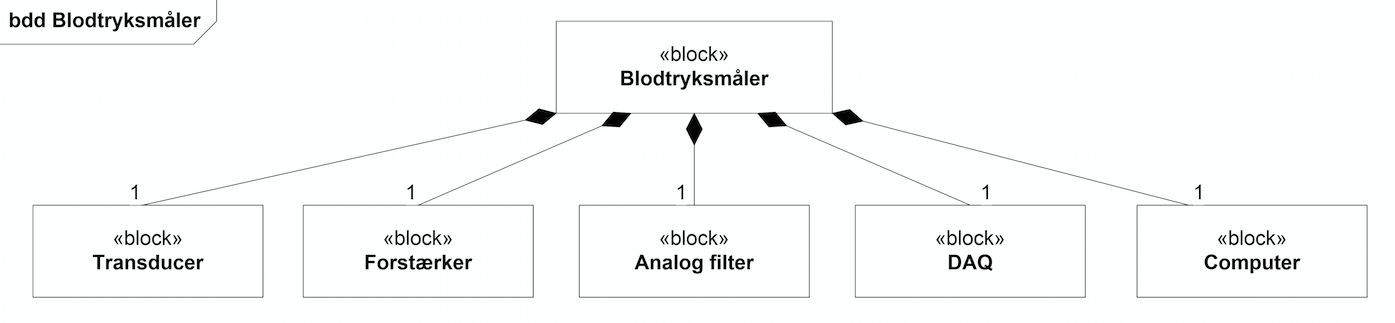
\includegraphics[width=1\textwidth]{Figurer/BDD}
	\caption{Blokdiagram for blodtryksmåler systemet.}\label{labelpic}
\end{figure}
\\Ud af blokdiagrammet kan man se at blodtryksmåler systemet består af en transducer, en forstærker, et analogt filter, en DAQ og en computer.
\\
\begin{figure}[h]
	\centering
	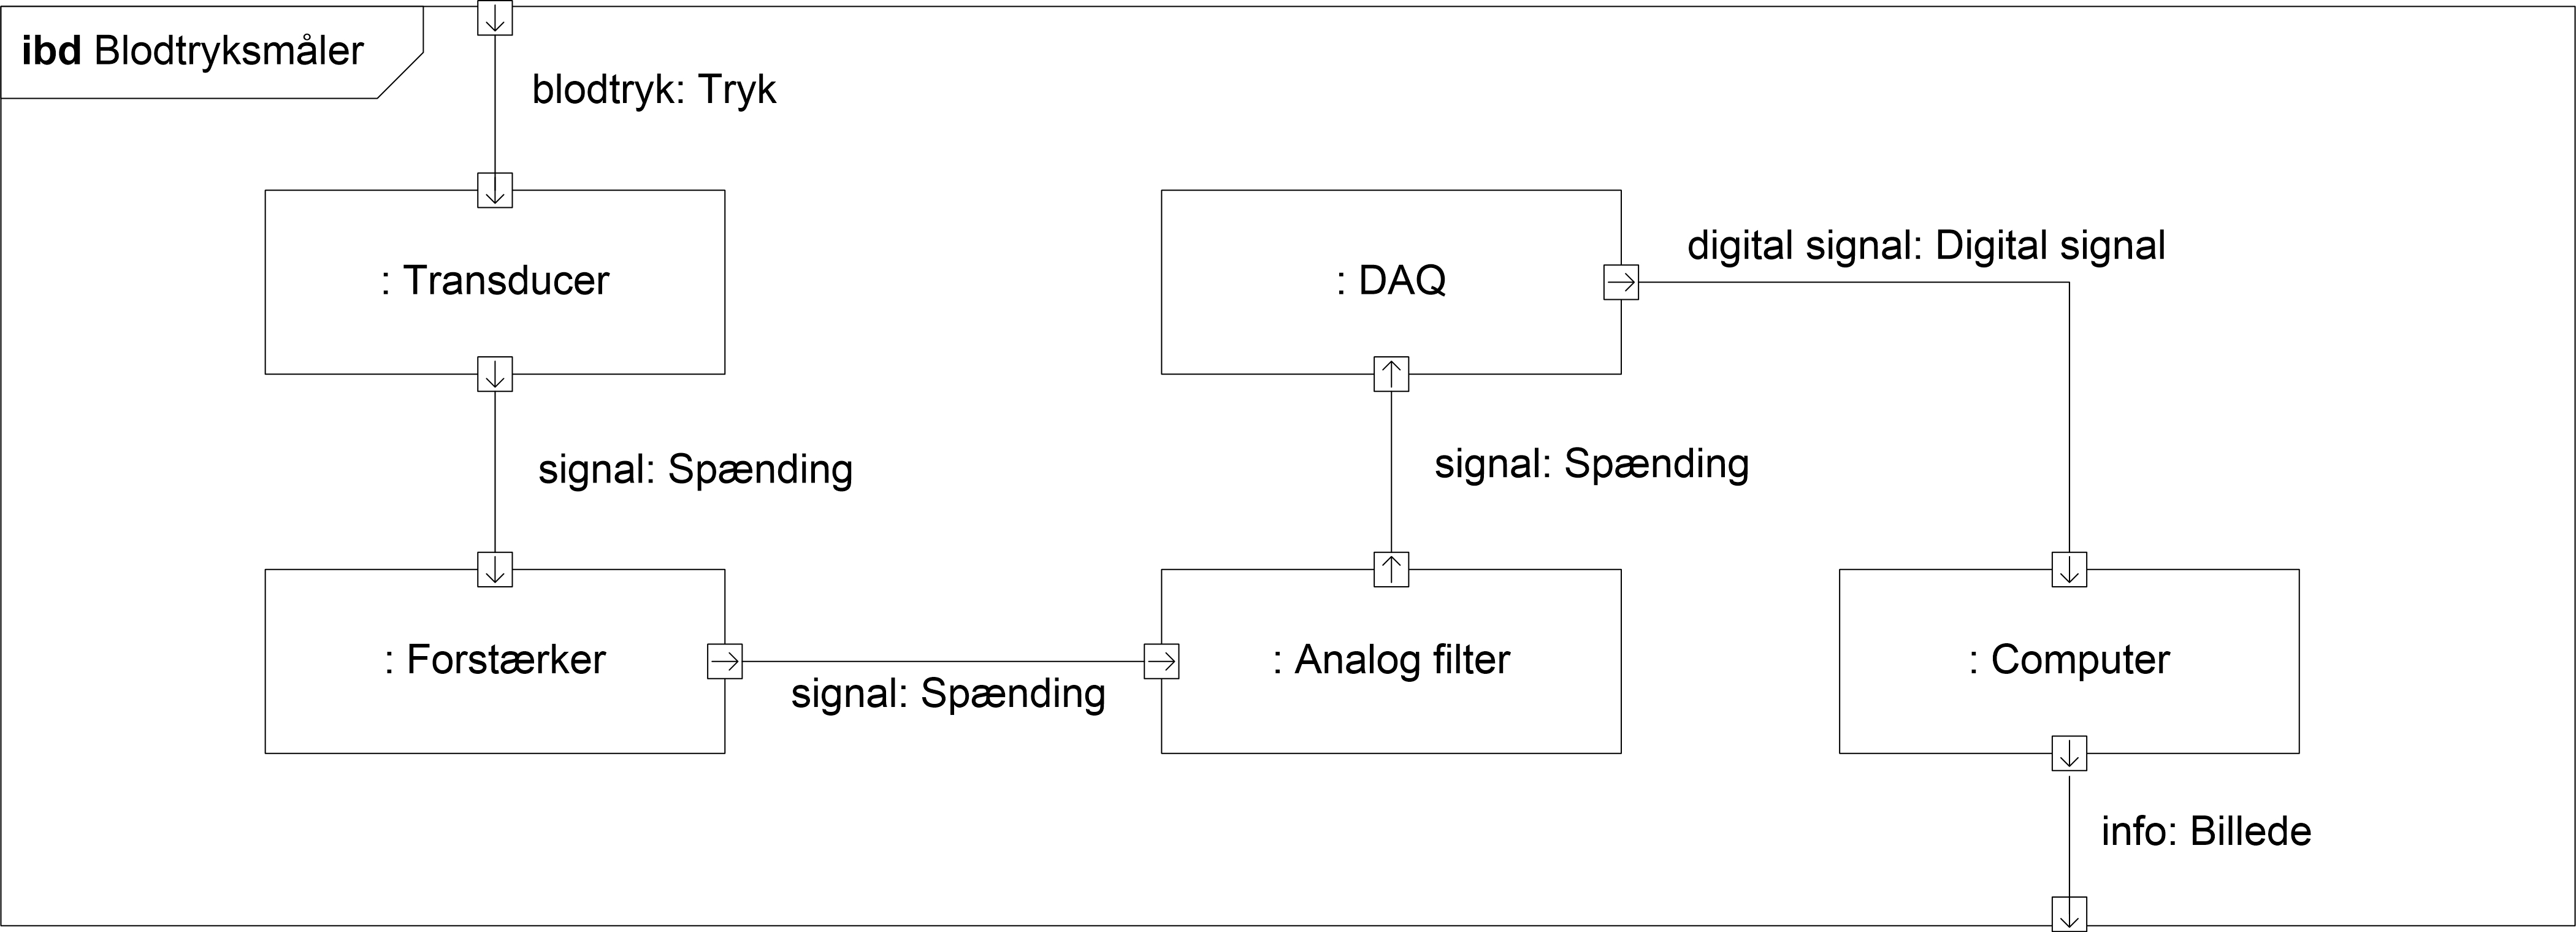
\includegraphics[width=1\textwidth]{Figurer/IBD}
	\caption{Internt blok diagram for blodtryksmåler systemet.}\label{labelpic}
\end{figure}
\\Ud af det interne blok diagram kan ses det at blodtrykket i form af det målte tryk kommer ind i transduceren. Transduceren som omformer det målte tryk til et spændingssignal, sender signalet vidre til forstærkeren. Fra forstærkeren sendes signalet over i det analoge filter og derfra ind i DAQ'en. Endeligt sendes det digitale signal fra DAQ'en over i en computer, der fortolker signalet som et billede, der vises til omverdenen.








\subsection{Grænseflader}

\section{Software arkitektur}


\subsubsection{Trelagsmodellen}

\subsection{GUI}

\subsection{UML klassediagram}


\subsection{Appliktationsmodel}
 

\subsubsection{Domænemodel}

\subsubsection{Sekvensdiagram}

\subsubsection{Opdateret Klassediagram}

\section{Software implementering}
 
\subsection{Visning af EKG-signal}

\subsection{Analyse}

\subsection{Testprogram}

\subsection{Lagring i database} 

\subsubsection{Offentlig database}

\subsubsection{Privat database}







